\section{A Running Example: DrawableDeck}~\label{sec:overview}
This section illustrates the features of our model for
resolving unintentional method conflicts. As mentioned before, such a
case arises when two inherited methods happen to have the same
signature, but with different semantics and functionality. This
situation is troublesome for programmers that use multiple
inheritance. Below we illustrate with a running example called
\lstinline|DrawableDeck|, which models a drawable deck of cards. 
Note that we use a Java-like syntax
throughout the paper, and all types are defined with the keyword
``\lstinline|interface|''. The concept is closely related to Java 8
interfaces with default methods~\cite{bono14} and traits. For simplicity, an interface in our model has
the following characteristics:
\begin{itemize}
  \item It allows multiple inheritance.
  \item Every method is either abstract or implemented to represent a behavior (like Java 8 default methods). 
  \item The \lstinline|new| keyword is used to instantiate an interface.
\end{itemize}
Furthermore, similarly to traits or Java 8 with default methods,
interfaces cannot have state.

%In the remainder of this section we show three problems that arize 
%from unintentional method conflicts. The first two problems 

%%for simplicity, our examples and formalization do not deal with state at
%%this stage. %%, but that should not block our discussions below.

\subsection{Problem 1: Unintentional Method Conflicts}
Suppose that two components \lstinline|Deck| and \lstinline|Drawable| 
have been developed in a system. \lstinline|Deck| represents a deck
of cards and defines a method \lstinline|draw| for drawing a card from the
deck.  \lstinline|Drawable| is an interface for graphics that
can be drawn and also includes a method called \lstinline|draw| for
visual display. For simple illustration, the default implementation of
\lstinline|draw| in \lstinline|Drawable| only creates a blank canvas
on the screen, while the \lstinline|draw| method in \lstinline|Deck| simply
prints out a message.

\vspace{3pt}\begin{lstlisting}
interface Deck {
  void draw() { // draws a card from the Deck
    println("Draw a card.");
  }
}

interface Drawable {
  JFrame draw() { // draws something on the screen
    JFrame frame = new JFrame();
    frame.setVisible(true);
    return frame;
  }
}
\end{lstlisting}\vspace{3pt}
Note that the two \lstinline|draw| methods have the same names and parameter types,
but the return types can be different. In \lstinline|Deck|,
\lstinline|draw| uses \lstinline|println|, which is a
library function. 
The method returns \lstinline|void|. Note that \lstinline|void| is
unsupported in our formalization, but we could have also defined an interface called \lstinline|Void|
and return an object of that type instead. For the method \lstinline|draw| in
\lstinline|Drawable|
the program has to create a blank canvas by \lstinline|JFrame|, which
is a pre-defined type.
\begin{comment}
\vspace{3pt}\begin{lstlisting}
interface JFrame {
  void setVisible(boolean b) {...}
  ...
}
\end{lstlisting}\vspace{3pt}
\end{comment}
Now, a programmer is designing a
card game with a GUI. He may want to draw a deck on the screen, so he defines a drawable
deck using multiple inheritance:

\vspace{3pt}\begin{lstlisting}
interface DrawableDeck extends Drawable, Deck {...} 
\end{lstlisting}\vspace{3pt}
The point of using multiple inheritance is for composing the features from various 
components and to achieve code reuse, as supported by many mainstream OO
languages. Nevertheless at this point, languages like Java simply treat the two \lstinline|draw| methods
as the same, and hence they throw a compile error on \lstinline|DrawableDeck| about the conflict, though accidentally.

Now one may quickly come up with a workaround, which is to create a new \lstinline|draw| method in \lstinline|DrawableDeck| to
explicitly override the old ones. However, the two conflicting methods
have totally different functionalities. Therefore merging
them into one does not make any sense. This non-solution will hide the
old methods and break independent extensibility. 

\paragraph{{\bf Potential Fixes:}}
There are several other workarounds
that come to our mind. We briefly discuss those potential fixes and
workarounds next:
\begin{itemize}
  \item \textbf{I. Delegation.} As an alternative to multiple inheritance,
  delegation can be used by introducing two fields (or field methods) with
  \lstinline|Drawable| type and \lstinline|Deck| type,
  respectively. This avoids method conflicts. Nevertheless, it is known
  that using delegation makes it hard to correctly maintain
  self-references in an extensible system and also
  introduces a lot of boilerplate code.
  \item \textbf{II. Refactor Drawable and/or Deck to rename the methods.} If
  the source code for \lstinline|Drawable| or \lstinline|Deck| is available
  then it may be possible to rename one of the \lstinline|draw|
  methods. However this approach is non-modular, as it requires 
  modifying existing code, and may not be possible if code is unavailable.
  \item \textbf{III. Method exclusion/renaming in traits.} Some trait models
  support method exclusion/renaming. Those features
   can eliminate conflicts, although most
  programming languages do not support them. In a traditional OO system,
  they can break the subtyping relationship. Moreover, in
  contrast with exclusion, renaming can indeed preserve both conflicting
  behaviours, however, it is cumbersome in practice, as introducing new
  names can affect other code blocks.
  \item \textbf{IV. Static dispatch.} Some other languages like C++ have
  direct support for the triangle inheritance. For instance, C++ allows both
  conflicting methods to coexist, and resolves the ambiguity by static dispatch:
  \vspace{3pt}\begin{lstlisting}[language=c++]
  class Deck { public: void draw() {...} };
  class Drawable { public: JFrame draw() {...} };
  class DrawableDeck : public Drawable, public Deck {};
  
  // in main
  DrawableDeck d;
  d.Deck::draw(); // prints the message
  \end{lstlisting}\vspace{3pt}
\end{itemize}

\bruno{Why have we eliminated problem 2 and included it in Problem 1?
Also why are we not showing how to actually solve it with our approach
now? I what we had previously made more sense. Please finish up this
section; show our solution, mention that is is quite similar (and
inspired by C++), but finish it saying that there are other problems
that C++ does not address.}
\subsection{Problem 2: Dynamic Dispatching}
So far it seems that static dispatch is the simplest and most straightforward approach,
as long as the language model accepts unintentionally conflicting methods. However, dynamic
dispatching appears to be more common in OO programming in order for code reuse. Following the previous example,
we reimplement \lstinline|Deck| with more features:

\vspace{3pt}\begin{lstlisting}
interface Deck {
  void draw() {...}
  void shuffle() {...}
  void shuffleAndDraw() { shuffle(); draw(); }
}
\end{lstlisting}\vspace{3pt}
Here \lstinline|shuffleAndDraw| is a typical method that invokes \lstinline|draw| in its definition. Ideally,
we want that invocation to be dynamically dispatched. This is important, because a programmer may define a subtype
of \lstinline|Deck| and override the method:

\vspace{3pt}\begin{lstlisting}
interface SafeDeck extends Deck {
  boolean isEmpty() {...}
  void draw() { // overriding
    if (isEmpty()) println("The deck is empty.");
    else println("Draw a card");
  }
}
\end{lstlisting}\vspace{3pt}
With static dispatch, we have to copy the \lstinline|shuffleAndDraw| code into \lstinline|SafeDeck|,
for the adaptation to the new \lstinline|draw|. Yet dynamic dispatching immediately saves us from the duplicate work,
since the method becomes automatically adaptive. Nevertheless, as seen before, dynamic dispatch would take us back to problem
1, for instance, when we
have the UML in Figure~\ref{fig:drawableloggingdeck} and the following code:

\begin{figure*}[t]
	\saveSpaceFig
	\centering
	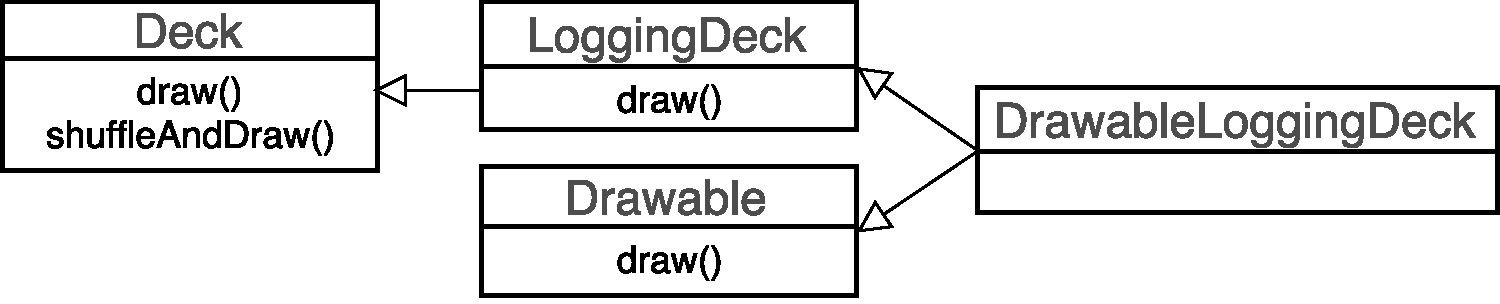
\includegraphics[height=2cm]{pics/DrawableLoggingDeck.pdf}
	\caption{UML graph for \lstinline|DrawableLoggingDeck|.}\label{fig:drawableloggingdeck}
	\saveSpaceFig
\end{figure*}

\vspace{3pt}\begin{lstlisting}
interface DrawableSafeDeck extends Drawable, SafeDeck {}

// main program
DrawableSafeDeck d = new DrawableSafeDeck();
d.shuffleAndDraw(); // ambiguous draw if dynamically dispatched
\end{lstlisting}\vspace{3pt}
From \lstinline|DrawableSafeDeck|'s point of view, the \lstinline|draw| method seems ambiguous. But ideally we would
like \lstinline|shuffleAndDraw| to invoke \lstinline|SafeDeck.draw| because they belong to the same branch. Hence it
seems that we choose dynamic dispatch but also make use of some static type information. Note that this problem can be
solved by the C++ code below:
\vspace{3pt}\begin{lstlisting}
class Deck { public: virtual void draw() {...} ... };
class Drawable {...};
class SafeDeck : public Deck { public: virtual void draw() {...} ... };
class DrawbaleSafeDeck : public Drawable, public SafeDeck {};

// in main
DrawableSafeDeck d;
d.shuffleAndDraw();
\end{lstlisting}\vspace{3pt}
By putting ``\lstinline|virtual|'' in front of every method signature, we are enforcing dynamic dispatch in C++.\\

\noindent\textbf{Our solution:} inspired by that, we propose \textit{hierarchical dispatch} in our model
as the default method lookup algorithm. A \textit{hierarchical invocation}, or \textit{path invocation}, namely
\lstinline|e.I?m()|, is read as
``finding the most specific method \lstinline|m| along the path
\lstinline|I|''. Formally, the meaning of ``along the path \lstinline|I|'' is
that, if the result of hierarchical dispatch finds \lstinline|J.m()| for some \lstinline|J|, then such a \lstinline|J| must be a super type of \lstinline|e|'s dynamic type for sure, and \lstinline|J| must have a subtyping relation with \lstinline|I| (either \lstinline|J <: I| or \lstinline|J >: I|). Intuitively, the most specific \lstinline|m| must be from branch \lstinline|I|, but it can be an updated version after \lstinline|I| because of dynamic dispatch. The formal definition will be introduced later.

On the other hand, \lstinline|e.m()| where \lstinline|e| has static type \lstinline|I|, simply behaves the same as \lstinline|e.I?m()| in our model. Such a dispatching algorithm makes use of both the static type and the dynamic type of the receiver, so it is seemingly a combination of static and dynamic dispatch. Intuitively, the static type specifies one branch to avoid ambiguity, and the dynamic type finds the latest version on that branch. It may still introduce ambiguity when there are multiple paths from the static type to the dynamic type, and those paths cause conflicts. We disallow this kind of conflict to ensure unambiguity. That is to say, we do not allow two methods to override a same base method when they cause conflicts. This is natural, as they are just two versions of the same operation, hence it is no longer an ``unintentional'' conflict, but the diamond problem.

Back to the example, our code below just suffices to meet the expectation:
\vspace{3pt}\begin{lstlisting}
interface Deck {
  void draw() {...}
  void shuffle() {...}
  void shuffleAndDraw() { shuffle(); draw(); }
}
interface Drawable {...}
interface SafeDeck extends Deck {...}
interface DrawableSafeDeck extends Drawable, SafeDeck {}

// main program
new DrawableSafeDeck().shuffleAndDraw() // calls Deck.shuffle, and then SafeDeck.draw
\end{lstlisting}\vspace{3pt}\haoyuan{mention how the language syntax is different from our formalization. FHJ is only a subset.}
Note that the \lstinline|draw()| in \lstinline|shuffleAndDraw()| is short for \lstinline|this.draw()|, and is equivalent to \lstinline|this.Deck?draw()|. It is because the compiler is able to know that the receiver ``\lstinline|this|'' exactly has static type \lstinline|Deck|. Hence hierarchical dispatch eliminates ambiguity in a concise way.\\

\noindent\textbf{Comparison with C++:} as an industrial language, C++ is more practical and flexible to use with lots of features, for example, it handles fields and virtual inheritance, and it allows explicit casts. But the compilation is more or less complicated, and sometimes unclear to programmers, which affects its type safety and people's understanding. The compilation seems to look into the expressions and the real (runtime) types for ambiguity check in method dispatching, and sometimes the errors are thrown by the linker. In contrast, inspired by C++ we formalize the concept of hierarchical dispatch in our model, with type-checking rules and semantics. The compilation only cares about the type of the receiver in method invocation, but the rules ensure type soundness so that the evaluation never throws errors on a program that type-checks. C++ does not hold type soundness for unintentional method conflicts, it actually accepts the diamond inheritance, and only complains on bad invocations. Whereas our model forbids the diamond case, which derives a strong type-safe system, and there are more theoretical aspects in Section~\ref{sec:formalization}. \haoyuan{not sure if this paragraph makes sense or is correct. Needs refs.}

\subsection{Problem 3: Overriding on Individual Branches}\label{subsec:partialoverrides}

We have seen that hierarchical dispatch can dynamically find the latest implementation of a method from one path (or branch). But when
several branches are merged by triangle inheritance, there is usually demand for updating them separately. For example, someone plans to
reuse the other features of \lstinline|DrawableLoggingDeck|, but updates the \lstinline|draw| from \lstinline|Drawable| by setting the canvas
invisible. Unfortunately in traditional models, the merged branches cannot be separately overridden any longer, since overriding
will hide all branches and break coexistence. Modifying existing code is again unsatisfactory as it affects modularity.\\

\noindent\textbf{Our solution:} an additional feature of our model is \textit{hierarchical overriding}. It allows conflicting methods
to be overridden on individual branches, and hence offers independent extensibility. The above example can be easily realized by:
\vspace{3pt}\begin{lstlisting}
interface DrawableLoggingDeck2 extends DrawableLoggingDeck {
  void draw() override Drawable {
    JFrame frame = new JFrame("Canvas");
    frame.setVisible(false);
    ...
  }
}
// main program
DrawableLoggingDeck2 d = new DrawableLoggingDeck2();
d.Drawable::draw()      // calling draw in DrawableLoggingDeck2
\end{lstlisting}\vspace{3pt}
\textbf{Terminology} The \lstinline|draw| methods we saw before this example are called ``original methods'' in this paper, because they are originally defined in its interface.
In contrast, \lstinline|DrawableLoggingDeck2| defines a ``hierarchical overriding'' method. The difference is that traditional overriding overrides all branches by defining another original method, whereas hierarchical overriding only refines one branch.

In our model, triangle inheritance allows several original methods (branches) to coexist, and hierarchical dispatch first finds the most specific original method (branch), then it finds the most specific hierarchical overriding on that branch. A quick counter-example is when there are two hierarchical overriding methods on \lstinline|Drawable| in \lstinline|DrawableLoggingDeck2|, it leads to ambiguity. The compiler is supposed to forbid that during compile time.

Two rules for hierarchical overriding: it can only refine \textbf{original} methods, and cannot jump over original methods with the same signature. For instance, writing \lstinline|"void draw()| \lstinline|override Deck {...}"| is disallowed in \lstinline|DrawableLoggingDeck2|, because existing two branches are \lstinline|Drawable.draw| and \lstinline|LoggingDeck.draw|, while \lstinline|Deck.draw| is already covered. It does not really make sense to refine an old branch.

Similar to many OO languages, the model also allows \textit{super method invocation} in a method body. The invocation \lstinline|super.T::m()| will ignore all the subtypes of \lstinline|T|, and only look at \lstinline|T| together with its super interfaces. It should behave the same as \lstinline|new T().m()| in principle.